\documentclass{standalone}
\usepackage{tikz}
\begin{document}
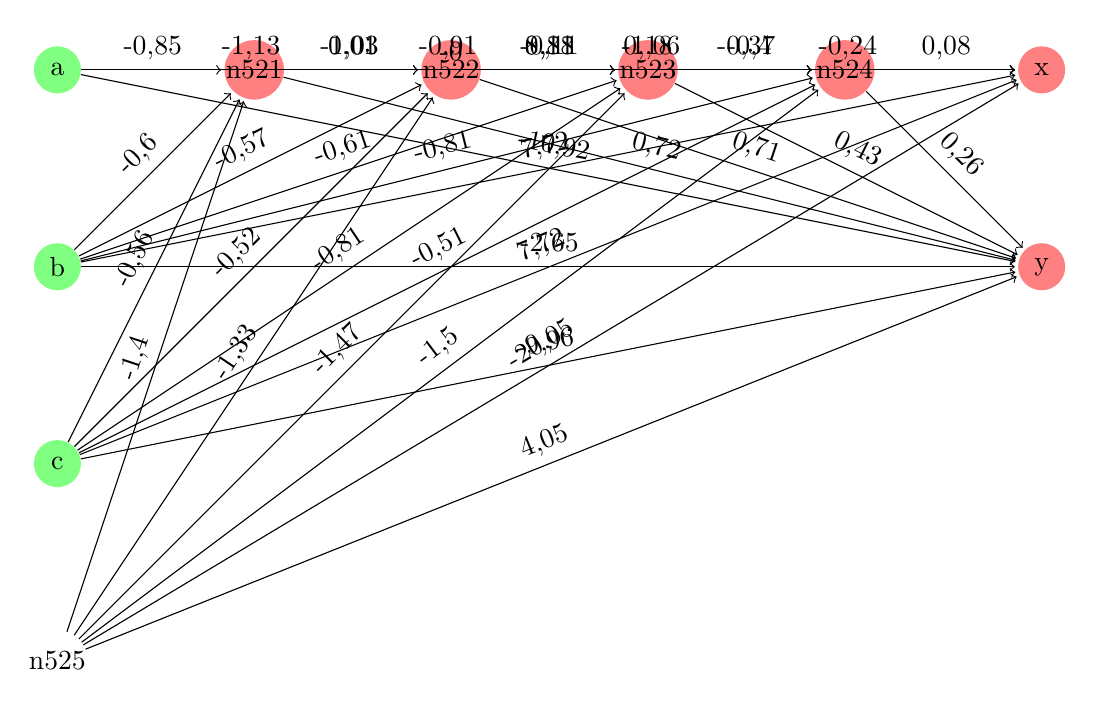
\begin{tikzpicture}[shorten >=1pt,->,draw=black!,node distance=2.5cm]
\tikzstyle{neuron}=[circle,fill=black!25,minimum size=17pt,inner sep=0pt]
\tikzstyle{constant}=[neuron, fill=white!50];
\tikzstyle{sigmoid}=[neuron, fill=red!50];
\tikzstyle{identity}=[neuron, fill=green!50];
\node [identity] (a) {a};
\node [identity,below of=a] (b) {b};
\node [identity,below of=b] (c) {c};
\node [constant,below of=c] (n525) {n525};
\node [sigmoid,right of=a] (n521) {n521};
\node [sigmoid,right of=n521] (n522) {n522};
\node [sigmoid,right of=n522] (n523) {n523};
\node [sigmoid,right of=n523] (n524) {n524};
\node [sigmoid,right of=n524] (x) {x};
\node [sigmoid,below of=x] (y) {y};
\path[every node/.style={sloped,anchor=south,auto=false}]
(n522) edge node {0,71} (y)
(n522) edge node {-0,4} (x)
(n522) edge node {0,18} (n524)
(n522) edge node {-0,11} (n523)
(n521) edge node {-1,06} (x)
(n521) edge node {0,72} (y)
(n521) edge node {-0} (n523)
(n521) edge node {0,01} (n522)
(n521) edge node {0,18} (n524)
(n524) edge node {0,26} (y)
(n524) edge node {0,08} (x)
(n523) edge node {-0,24} (x)
(n523) edge node {0,43} (y)
(n523) edge node {-0,37} (n524)
(n525) edge node {4,05} (y)
(n525) edge node {-1,4} (n521)
(n525) edge node {-20,05} (x)
(n525) edge node {-1,5} (n524)
(n525) edge node {-1,33} (n522)
(n525) edge node {-1,47} (n523)
(c) edge node {7,72} (x)
(c) edge node {-0,56} (n521)
(c) edge node {-9,96} (y)
(c) edge node {-0,81} (n523)
(c) edge node {-0,52} (n522)
(c) edge node {-0,51} (n524)
(b) edge node {-2,65} (y)
(b) edge node {7,72} (x)
(b) edge node {-0,57} (n522)
(b) edge node {-0,6} (n521)
(b) edge node {-0,81} (n524)
(b) edge node {-0,61} (n523)
(a) edge node {8,81} (x)
(a) edge node {-0,91} (n524)
(a) edge node {-0,85} (n521)
(a) edge node {-10,92} (y)
(a) edge node {-1,03} (n523)
(a) edge node {-1,13} (n522)
;\end{tikzpicture}
\end{document}